%!TEX root = ../main.tex

% NOTES:
%   * There is a shift to accelerator design
%   * CPUs are inefficient
%   * Fixed accelerators are hard to program
%   * Alternative is FPGA/CGRA
%   * There are challenges with programming FPGA/CGRA
%   * HLS is one solution

%


\section{Abstraction Levels}

The growing capabilities of silicon technology over the previous decades has forced design methodologies and tools to move to higher levels of abstraction
In order to explain the relationship between different design methodologies on
different abstraction levels, we will use the Y-Chart~\cite{walker_1985_y_model} to explain differences between different design tools and different design methodologies in which these tools were used.

\begin{figure}[h]
    \centering
    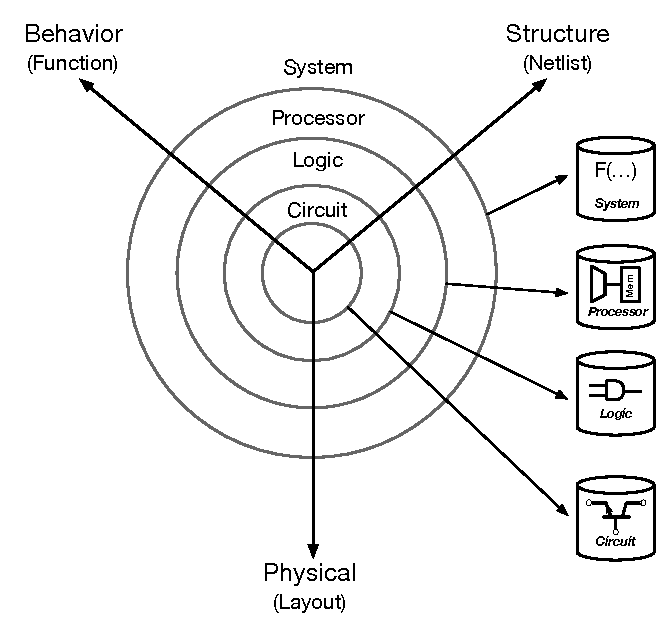
\includegraphics[width=0.5\textwidth]{figures/Introduction/Y-Chart.pdf}
    \caption{Y-Chart}
    \label{fig:y-chart}
\end{figure}

Y-Chart divides design representation into three domains:1)Behavioral, it can also called functionality and specification, 2)Structural, also called netlist or a block diagram and 3)Physical, usually called layout or board design. Behavior represents a design as a black-box but it describes the output base on inputs over time. What behavior representation doesn't specify is how the black-box is structured or how to build the black-box. This is the task of structural representation. In this specification, black-box is represented as a set of components and connections. While, it's possible to drive the behavior of black-box from its components and its connections but understanding the behavior can be very difficult since it is obscured by the details of each component and connection.
Eventually, physical design describe different dimension of each component.

The Y-chart also defines multiple level of abstractions for a design by drawing concentric circles on the Y. Typically, four levels are used: system, processor, logic and circuit levels.
The name of each abstraction level is derived from the types of the components generated on that abstraction level.
For instance, on the processor level, we generate standard and custom processors, or special-hardware components such as memory controllers, arbiters, brides and various interface components. At the higher level, system level, we design standard or embedded systems consisting of processors, memories, buses, and other processor components.

Let's look at binary counter as an example. In this example at the algorithmic-level, we only know that at every cycle the input value will be increased by one and the output in the next cycle would be the input plus one.
At the next lower level, we understand that to carry out this function some sort of register is needed to hold the value of the counter.
We can state this idea using a register transfer statement such as $AC \leftarrow AC + 1$.
On the structural side, the register consists of gates and flip-flops, which themselves consist of transistors.

On each abstraction level, we need a library of components to be used in building \emph{the structure} for a given \emph{behavior}.
This process of converting the given behavior into a structure for a given haviour is called \textbf{synthesis}.
Once a structure is defined and verified, we can proceed to the next lower abstraction level by further synthesizing each of the components in the structure.
On the other hand, if each component in the library is given with its structure and
the physical implementation, we can proceed with physical design.
Thus each component in the library may have up to three different models representing
three different axes in the Y-Chart: behavior or function; structure, which
contains the components from the lower level of abstraction; and the physical.

In the rest of this chapter we focus on the first two level of abstractions, \textit{Processr} and \textit{System}.
Fortunately, all three models for each component are not typically needed most of the time.
Most of the methodologies presently in use perform design or synthesis on the system and processor levels, where every system component except standard processors and memories is synthesized to the logic level, before the physical design is performed on the logic level.
Therefore, for the top three abstraction levels, we only need a functional model of each component with estimates of the key metrics such as performance, delay, power, cost, size, reliability, testability, etc.
Once the design is represented in terms of logic gates and flip-flops, we can use standard cells for each logic component and perform layout placement and routing.
On the other hand, some components on the processor-and-system levels may be obtained as IPs and not synthesized.
Therefore, their structure and physical design are known, at least partially, on the level higher than logic level.
In that case, the physical design then may contain components of different sizes and from different levels of abstraction.

We first explain behavioral model and structural model of each level of abstraction. And then we explain the procedure or moving from behavioral domain to procedural domain.


\section{Processor-Level Behavioral Model}
\label{sec:processor_level_behavioral_model}

On the processor level, we define and design computational components or processing elements (PEs).
Each PE can be a dedicated or custom component that computes some specific functions, or it can be a general or standard PE that can compute any function specified in some standard programming language.
The functionality or behavior of each PE can be specified in several different ways.

In the basic implementation of PEs, their functionality can be specified with mathematical expressions or formulas.
But there is no limitation on what the functionaly of a PE can be.
Therefore, we can expand the functionality of a PE and specify it with an algorithm in some \textit{programming language}.
If we want to go beyond a mathematical expression, we solution is to use Finite State Machines (FSMs).
A FSM is defined with a set of states and a set of transitions from state to state, which are taken when some input variables reach the required value. Furthermore, each FSM generates some val- ues for output variables in each state or during each transition. A FSM model can be made clock-accurate if each state is considered to take one clock cycle. In general, a FSM model is useful for computations requiring several hundred states at most.

This FSM model use standard integer or floating-point variables and computing their values in each state or during each transition by a set of arithmetic expressions or programming statements.
For example, Figure~\ref{fig:fsm_model} shows a FSM with three states, S1, S2, and S3, and with arcs representing state changes under different inputs.
Each state executes a computation represented by one or more arithmetic expressions or programming statements.
For example, in state S1, the FSM in Figure~\ref{fig:fsm_model} computes two functions, $x = |a|$ and $y = |b|$, and in state S3 it computes the function $z = max (x, y)$.
A FSM model is usually not clock-accurate since computation in each state may take more than one clock cycle.
Therefore, using FSM model to represent computation expressed by programming languages like C is not adequet.

\begin{figure}[h]
    \centering
    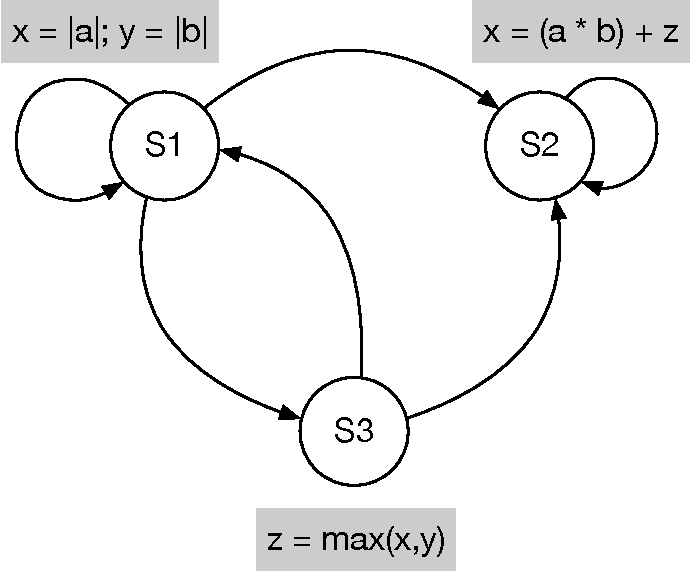
\includegraphics[width=0.4\textwidth]{figures/Introduction/FSM.pdf}
    \caption{FSM model}
    \label{fig:fsm_model}
\end{figure}


In general, programming languages consist of \code{if} statements, loops, and expressions.
An \code{if} statement has two parts, then and else, in which then is executed \code{if} the conditional expression given in the \code{if} statement is true, otherwise the else part is executed.
In each of the then or else parts, the \code{if} statement computes \emph{a set of expressions called a Basic Block (BB)}.
The \code{if} statement can also be used in the loop construct to represent loop iterations, which are executed as long as the condition in the \code{if} statement is true.
Therefore, any programming-language code can be represented by a Control-Data Flow Graph (CDFG) consisting of \code{if} diamonds, which represent \code{if} conditions, and BB blocks, which represent computation [151].
Figure~\ref{fig:dcfg_model} shows such a CDFG, this one representing a loop with an \code{if} statement inside the loop iteration.
In each iteration, the loop construct executes BB1 and BB2 or BB3 depending on the value of \code{if} statement.
At the end, the loop is exited if all all iterations are executed.

A CDFG shows explicitly the control dependencies between loop statements, if statements, and BBs, as well as the data dependences among operations inside a BB.
It can be converted to a FSM by assigning a state to each BB and one state for the computation of each if conditional.
Note that each state in such a FSM may need several clock cycles to execute its assigned BB or if condition.

\begin{figure}[h]
    \centering
    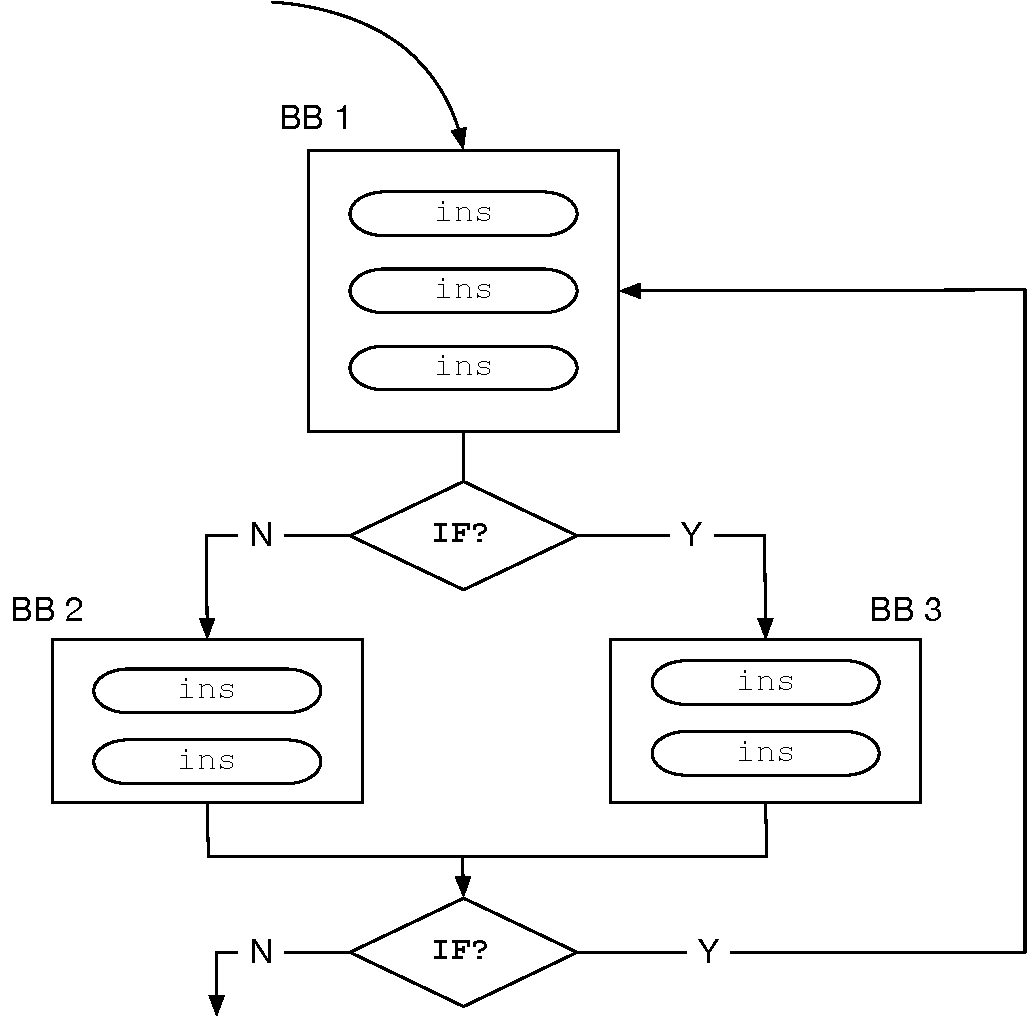
\includegraphics[width=0.55\textwidth]{figures/Introduction/CFG.pdf}
    \caption{FSM model}
    \label{fig:dcfg_model}
\end{figure}

\section{Processor-Level Structural Model}

A processor’s behavioral model, whether defined by a program in C, CDFG, FSM, or by an IS, can be implemented with a set of register-transfer components; such a structural model usually consists of a controller and a datapath like general purpose processors.
A datapath consists of a set of storage elements (such as registers, register files, and memories), a set of functional units (such as ALUs, multipliers, shifters, and other custom functional units), and a set of busses.
All of these register-transfer components may be allocated in different quantities and types and connected arbitrarily through busses or a network-on-chip (NOC).
Each component may take one or more clock cycles to execute, each component may be pipelined, and each component may have input or output latches or registers.
In addition, the entire datapath can be pipelined in several stages in addition to components being pipelined by themselves.
The choice of components and datapath structure depends on the metrics to be optimized for particular implementation.

The controller defines the state of the processor clock cycle per clock cycle and issues the control signals for the datapath accordingly.
The structure of the controller and its implementation depends on whether the processor is a standard processor (such as Xeon, ARM, or a DSP) or a custom-design processor or Intellectual Property (IP) function specifically synthesized for a particular application and platform.
For instance, in the case of a standard processor, the controller is programmable with a program counter (PC), and an address generator (AG) that defines the next address to be loaded into the PC.
In the case of specific custom processors, the controller can be implemented with programmability concepts typical of standard processors, and control signal generation of IP implementations like CGRAs.

\begin{figure}[h]
    \centering
    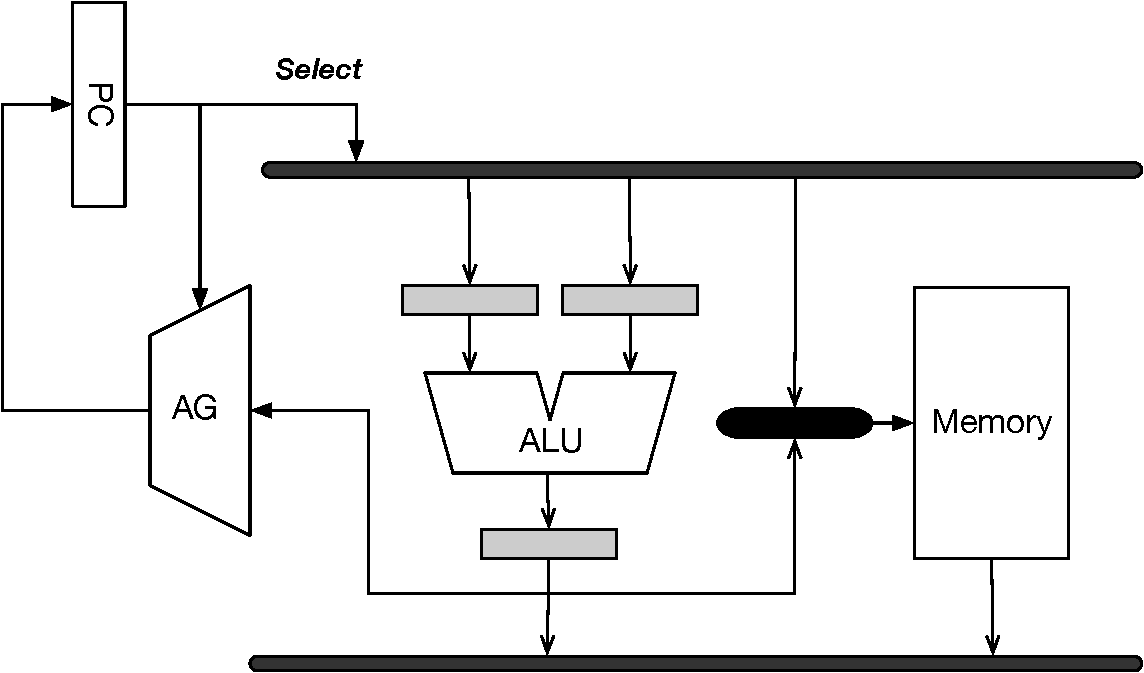
\includegraphics[width=0.6\textwidth]{figures/Introduction/Processor_Structure.pdf}
    \caption{Processor structure model}
    \label{fig:proc_structure}
\end{figure}



\section{Processor-Level Synthesis}

Synthesis of standard processors starts with the instruction set (IS) of the processor.
In order to achieve the highest processor performance this process is done manually since standard processors try to achieve the highest performance and minimal power consumption at minimal cost.
The second reason for synthesizing processors manually is to minimize the design size and therefore fabrication cost for high-volume production.
In contrast, the design or synthesis of a custom processor or a custom IP starts with the C code of an algorithm, which is usually converted to the corresponding CDFG or FSMD model before synthesis and ends up with a custom processor containing the number and type of components connected as required by the given behavioral model.
This generation is usually called high-level synthesis or register-transfer synthesis or occasionally just processor synthesis.
Selecting components and the structure of a PE and \emph{defining register-transfer operations performed in each clock cycle is the task of processor-level synthesis.}

\begin{figure}[h]
    \centering
    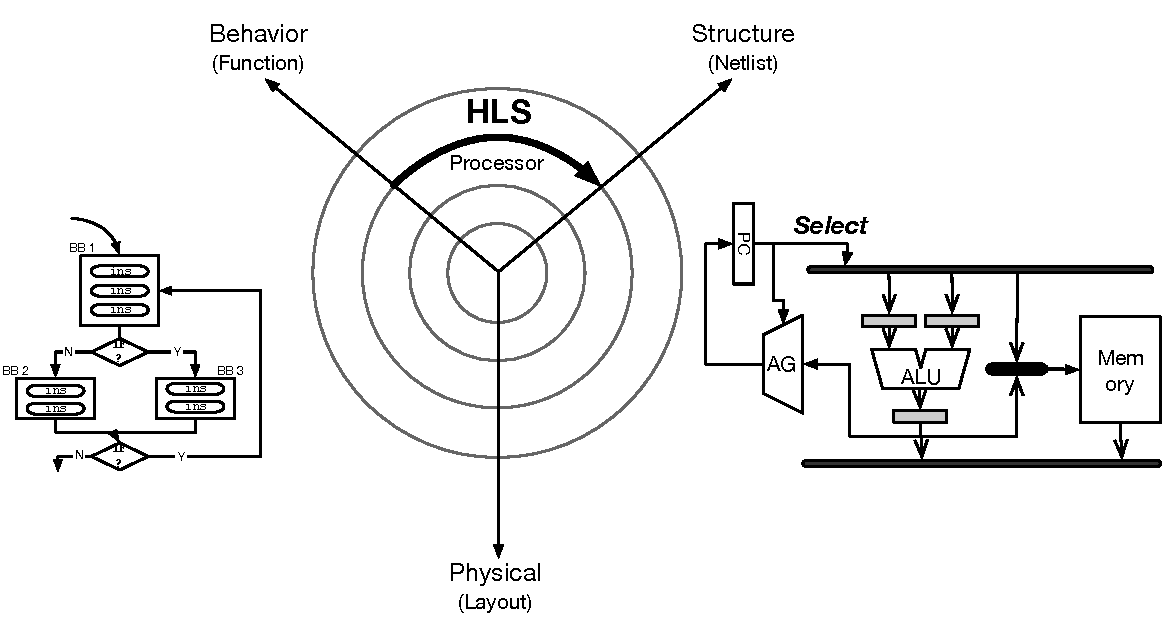
\includegraphics[width=0.9\textwidth]{figures/Introduction/processor-synthesis.pdf}
    \caption{High-Level Synthesis (HLS)}
    \label{fig:proc_synthesis}
\end{figure}


\section{System-Level Model}

Processor-level behavioral models such as the CDFG can be used for specifying a single processor, but will not suffice for describing a complete system that consist of many communicating processors.
A system-level model must represent multiple processes running in parallel in SW and HW.
The easiest way to do this is to use a model which retains the concept of states and transitions as in a FSM but which extends the computation in each state to include processes or procedures written in a programming language such as C/C++.
Furthermore, in order to represent a many-processor platform working in parallel or in pipelined mode, we must introduce concurrency and pipelining.
Since processes in a system run concurrently, we need a synchronization mechanism for data exchange, such as the concept of a channel, to encapsulate data communication.
Also, we need a model which supports hierarchy, so as to allow designers to write complex system specifications without difficulty.
Figure~\ref{fig:task_graph} illustrates such a model of hierarchical sequential-parallel processes, which is
usually called a Process State Machine (PSM).
This particular PSM is a system-level behavior or system specification, consisting of processes P1 to P5.
The
system starts with P1, which in turn triggers process P2 if condition d is true, or
another process consisting of P3, P4, and P5 if condition d is not true. P3 and
P4 run sequentially and in parallel with P5, as indicated by the vertical dashed
line. When either P2 is finished or the sequential-parallel composition of P3,
P4, and P5 is finished, the execution ends.

\begin{figure}[h]
    \centering
    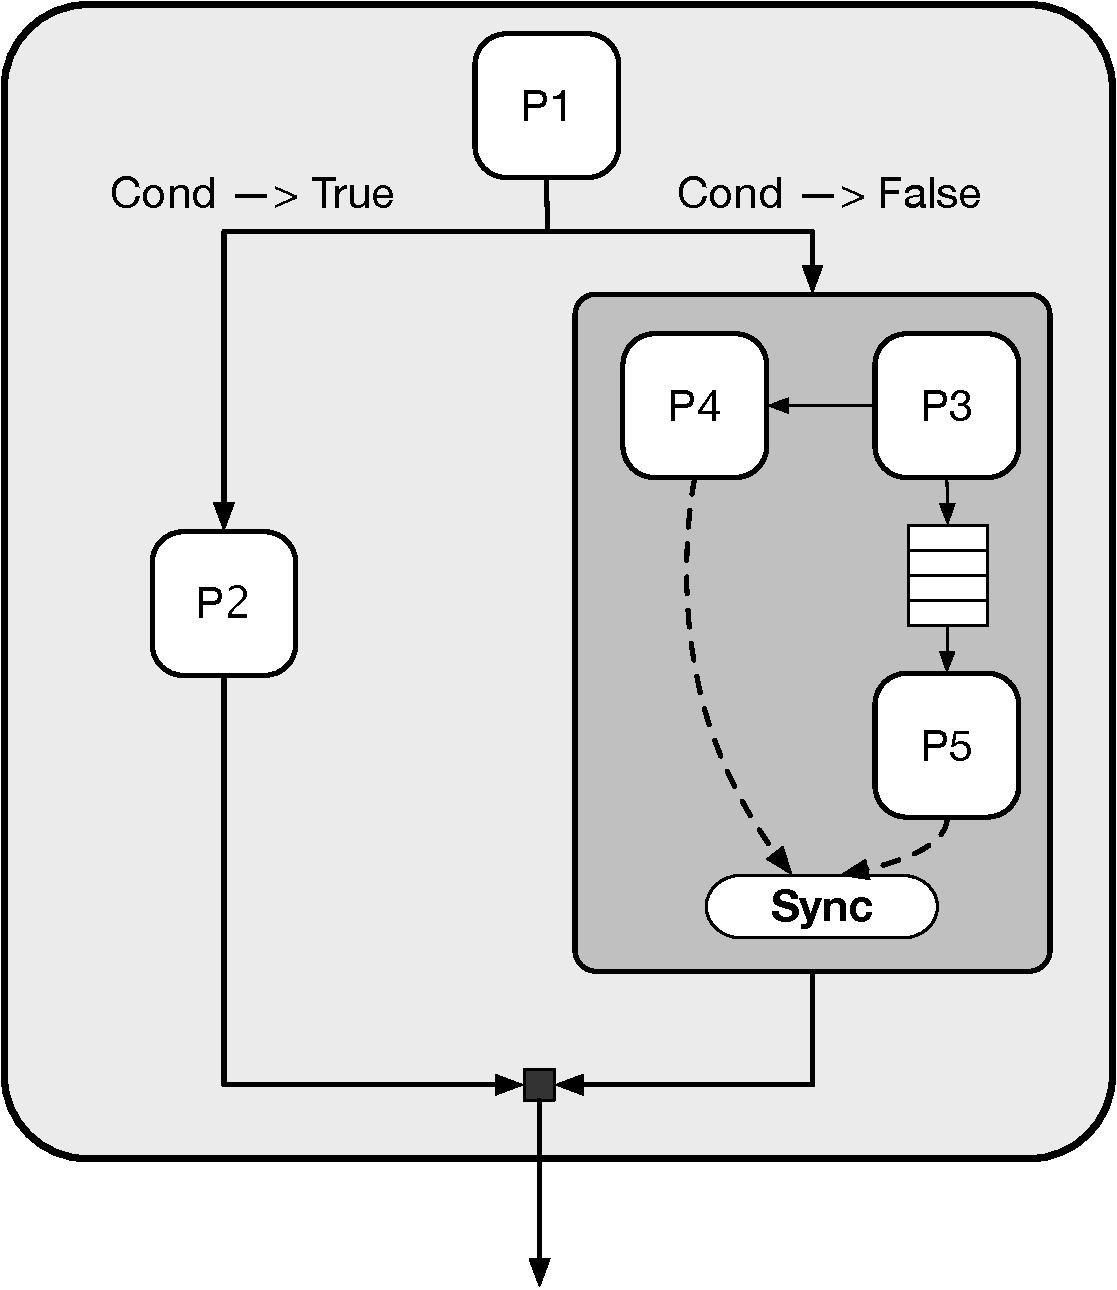
\includegraphics[width=0.4\textwidth]{figures/Introduction/Task_Graph.pdf}
    \caption{System behavioral model}
    \label{fig:task_graph}
\end{figure}


In the synthesis part we need to answer question like what is the memory model. How is the memory shared across different processes.



\subsection{Missing Semantics}
\label{sec:missing_semantics}

A big challenge in \emph{synthesising} is missing semantics. In many cases there are many different representation and design for a same behavioral model. But which model fits better in our design. 
As an example of this problem, we can look in ~\ref{fig:missing_semantics} at a simple case statement available in any hardware or system modeling language.
This type of case statement can be used to model a FSM in which every case such as X1,X2, ..., represents a state in which all its next states are de ned.
This type of case statement can also be used to model a look-up table, in which every case X1, X2, ..., indicates a location in the memory that contains a value in the table.
Therefore,  we can use the same case statement with the same variables and format to describe two completely different components.
Unfortunately, FSMs and look-up tables require completely different implementations:  a FSM can be implemented with a controller or with logic gates, while a look-up table is usually implemented with some kind of memory.
It is also possible to implement a FSM with a memory or a table using logic gates.
However, this would not bea very ef cient implementation, and it would not be acceptable to any designer.
So a model which uses case statements to model FSMs and tables is good for simulation but not for implementation because neither a designer nor a synthesis tool can determine which type of structure was described by the case statement.
The lesson is that contemporary modeling languages allow modelers to de-scribe the design in many different ways and to use the same description for different designs details. But for automatic refinement, synthesis, and veri cation, we need clean and unambiguous semantic which uniquely represents all the system concepts in a given model.  Such a clean semantic is missing from most of the simulation-oriented  languages.
In order to have well defined semantics, we need to introduce some form of formalism to models and modeling languages.


\begin{figure}[h]
    \centering
    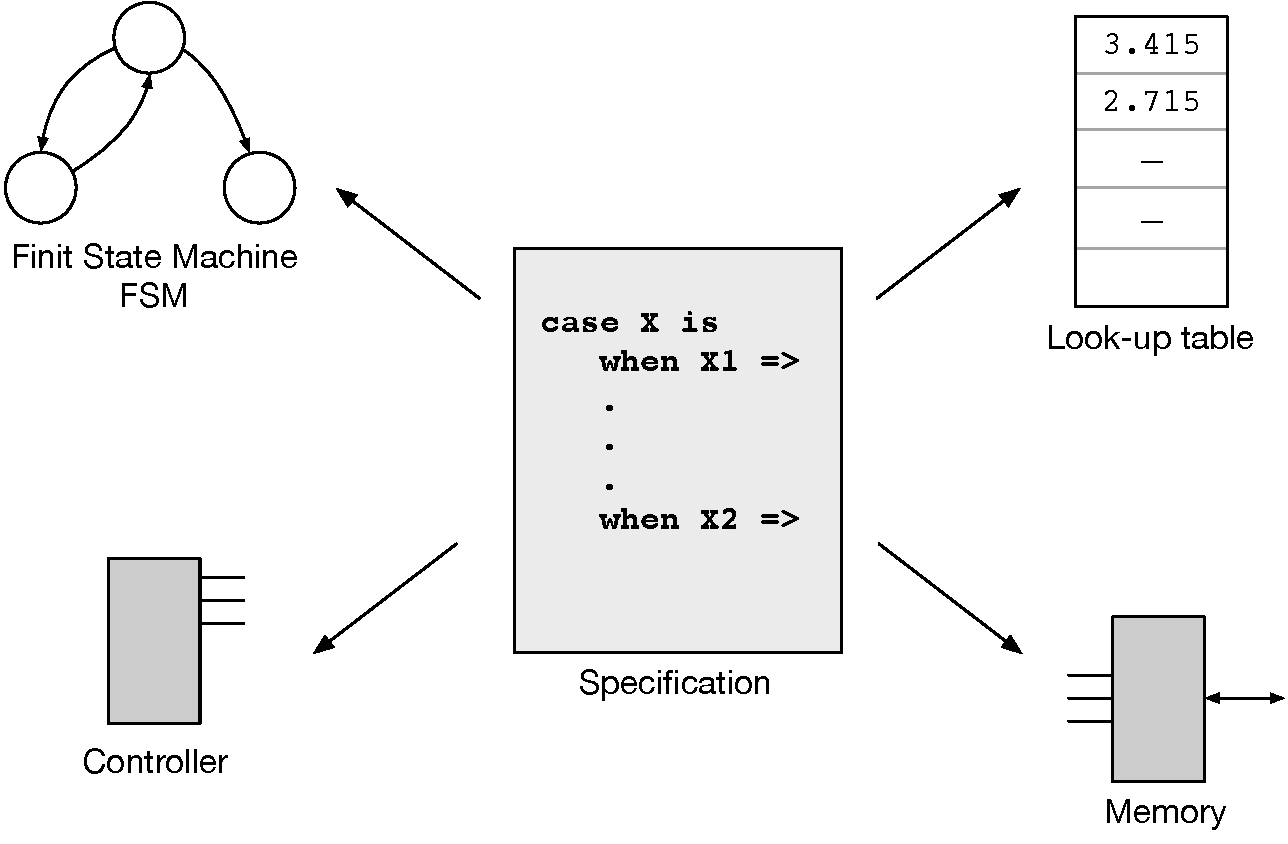
\includegraphics[width=0.7\textwidth]{figures/Introduction/Missing_Semantics.pdf}
    \caption{Missing Semantics}
    \label{fig:missing_semantics}
\end{figure}


\section{Design Search Exploration}
% * The last goal is to optimize the design

\section{Hardware Design Methodologies}

\paragraph{Method1:} Describe-and-Synthesize methodology (late 1980s to late 1990s).
The 1980s brought us tools for logic synthesis which have significantly altered design flow, since the behavior and structure of a design were both captured on the logic level.
Designers specified first what they wanted in Boolean equations or FSM descriptions, and then the synthesis tools generated the implementation in terms of a logic-level netlists.
In this methodology therefore, the behavior or function comes first, and the structure or implementation comes afterwards.
Moreover, both of these descriptions are simulatable, which is an marked improvement over Capture-and-Simulate methodology, because it permits much more efficient verification; it makes it possible to verify the descriptions’ equivalence since both descriptions can in principle be reduced to a canonical form.
However, today’s designs are too large for this kind of equivalence checking.
By the late 1990s, the logic level had been abstracted to the Register-Transfer Level (RTL) with the introduction of cycle-accurate modeling and synthesis.
Therefore, we now have two abstraction levels (RTL and logic levels) and two different models on each level (behavioral and structural).
However, the system gap still persists because there was not relation between RTL and higher system level.

\paragraph{Method2:}  The 1980s brought us tools for logic synthesis which have significantly altered design flow, since the behavior and structure of a design were both captured on the logic level.
Designers specified first what they wanted in Boolean equations or FSM descriptions, and then the synthesis tools generated the implementation in terms of a logic-level netlists.
In this methodology therefore, the behavior or function comes first, and the structure or implementation comes afterwards.
Moreover, both of these descriptions are simulatable, which is an marked improvement over Capture-and-Simulate methodology, because it permits much more efficient verification; it makes it possible to verify the descriptions’ equivalence since both descriptions can in principle be reduced to a canonical form.
However, today’s designs are too large for this kind of equivalence checking.

By the late 1990s, the logic level had been abstracted to the Register-Transfer Level (RTL) with the introduction of cycle-accurate modeling and synthesis.
Therefore, we now have two abstraction levels (RTL and logic levels) and two different models on each level (behavioral and structural).
However, the system gap still persists because there was not relation between RTL and higher system level.


\paragraph{Methode3:}
Specify, Explore-and-Refine methodology (early 2000s to present).
In order to close this gap, we must increase the level of abstraction from the RTL to the system level (SL) and to introduce a methodology that includes both SW and HW.
On the SL, we can start with an executable specification that represents the system behavior; we can then extend the system-level methodology to include several models with different details
that correspond to different design decisions. Each model is used to prove some system property: functionality, application algorithms, connectivity, communication, synchronization, coherence, routing, performance, or some design metric such as performance, power, and so on.
So we must deal with several models in order to verify the impact of design decisions on every metric starting from an executable specification down to the RTL and further to the physical design.
We can consider each model as a specification for the next level model, in which more implementation detail is added after more design decisions are made.
We can label this a Specify-Explore-Refine (SER) methodology [63, 100], in that it consists of a sequence of models in which each model is a refinement of the previous.
Thus SER methodology follows the natural design process in which designers specify the intent first, then explore possibilities, and finally refine the model according to their decisions.
SER flow can therefore be viewed as several iterations of the basic Describe-and-Synthesize methodology.

In order to explain about SER model first we overview the status of methodologies presently in use, their shortcomings, and how to upgrade them to the system level.

